% This file provides a template to format JASSS articles v.0.5, 2015-03-24

% In order to be compiled, the following packages should be installed in your system:
% graphicx,xcolor, booktabs,amsmath, ifthen, geometry, authblk, natbib, endnotes
 
 % Please use pdflatex

% The font used is Source Sans Pro, normally included in Tex Live and other  major LaTeX distributions
% Location at CTAN: http://www.ctan.org/tex-archive/fonts/sourcesanspro/
% See also: http://www.tug.dk/FontCatalogue/sourcesanspro/

%%%%%%%%%%%%%%%%%%%%%%%%%%%%%%%%%%%%%%%%%%%%%%

\documentclass{JASSS}
	
%%%%%%%%%%%%%%%%%%%%%%%%%%%%%%%%%%%%%%%%%%%%%%

% Editorial fields (to be set in case of publication)	
% Please leave this section untouched
%\doinum{10.18564/jasss.xxxx}
%\volume{xx}
%\issue{x}
%\article{x}
%\pubyear{20xx}
%\received{dd-mmm-yyyy}
%\accepted{dd-mmm-yyyy}
%\published{dd-mmm-yyyy}

%%%%%%%%%%%%%%%%%%%%%%%%%%%%%%%%%%%%%%%%%%%%%% 

% title, authors and affiliations	

\title{Population Synthesis with Quasirandom \\Integer Sampling}

%All authors should be included in the submission. To anonymise the submission, set to 'true' the \reviewcopy command below. However, before submitting  you can check that all the informations you entered are correct by temporarily setting it to 'false'. Please remember to set it back to 'true' before the submission.
\reviewcopy{true} 

\author[1]{Andrew P Smith}

% Subsequent author should be included using the following template. You can add more in case of need, just remember to appropriately set the corresponding number.  Please check the the authblk package documentation  in case of doubts

\author[1]{Robin Lovelace}
\author[1]{Mark Birkin}
\affil[1]{University of Leeds}

% email for the corresponding author
\email{a.p.smith@leeds.ac.uk}

%%%%%%%%%%%%%%%%%%%%%%%%%%%%%%%%%%%%%%%%%%%%%%

% NOTES. Please use endnotes. Notes should be placed after the main text and appendices and before the references. Also remember to uncomment the \theendnotes commands at the end of the document (just before the references)

%%%%%%%%%%%%%%%%%%%%%%%%%%%%%%%%%%%%%%%%%%%%%%

% REFERENCES should be included using the \citep, \citet, etc. commands provided by the natbib package

\usepackage{natbib}
	\setcitestyle{authoryear,round,aysep={}}
	
%%%%%%%%%%%%%%%%%%%%%%%%%%%%%%%%%%%%%%%%%%%%%%	

% EXTRA PACKAGES. Please place here any extra package you need along with your own command definitions
\usepackage{amssymb,amsmath}
\usepackage{hyperref}

\usepackage{color}
\usepackage{fancyvrb}
\newcommand{\VerbBar}{|}
\newcommand{\VERB}{\Verb[commandchars=\\\{\}]}
\DefineVerbatimEnvironment{Highlighting}{Verbatim}{commandchars=\\\{\}}
% Add ',fontsize=\small' for more characters per line
\usepackage{framed}
\definecolor{shadecolor}{RGB}{248,248,248}
\newenvironment{Shaded}{\begin{snugshade}}{\end{snugshade}}
\newcommand{\KeywordTok}[1]{\textcolor[rgb]{0.13,0.29,0.53}{\textbf{{#1}}}}
\newcommand{\DataTypeTok}[1]{\textcolor[rgb]{0.13,0.29,0.53}{{#1}}}
\newcommand{\DecValTok}[1]{\textcolor[rgb]{0.00,0.00,0.81}{{#1}}}
\newcommand{\BaseNTok}[1]{\textcolor[rgb]{0.00,0.00,0.81}{{#1}}}
\newcommand{\FloatTok}[1]{\textcolor[rgb]{0.00,0.00,0.81}{{#1}}}
\newcommand{\ConstantTok}[1]{\textcolor[rgb]{0.00,0.00,0.00}{{#1}}}
\newcommand{\CharTok}[1]{\textcolor[rgb]{0.31,0.60,0.02}{{#1}}}
\newcommand{\SpecialCharTok}[1]{\textcolor[rgb]{0.00,0.00,0.00}{{#1}}}
\newcommand{\StringTok}[1]{\textcolor[rgb]{0.31,0.60,0.02}{{#1}}}
\newcommand{\VerbatimStringTok}[1]{\textcolor[rgb]{0.31,0.60,0.02}{{#1}}}
\newcommand{\SpecialStringTok}[1]{\textcolor[rgb]{0.31,0.60,0.02}{{#1}}}
\newcommand{\ImportTok}[1]{{#1}}
\newcommand{\CommentTok}[1]{\textcolor[rgb]{0.56,0.35,0.01}{\textit{{#1}}}}
\newcommand{\DocumentationTok}[1]{\textcolor[rgb]{0.56,0.35,0.01}{\textbf{\textit{{#1}}}}}
\newcommand{\AnnotationTok}[1]{\textcolor[rgb]{0.56,0.35,0.01}{\textbf{\textit{{#1}}}}}
\newcommand{\CommentVarTok}[1]{\textcolor[rgb]{0.56,0.35,0.01}{\textbf{\textit{{#1}}}}}
\newcommand{\OtherTok}[1]{\textcolor[rgb]{0.56,0.35,0.01}{{#1}}}
\newcommand{\FunctionTok}[1]{\textcolor[rgb]{0.00,0.00,0.00}{{#1}}}
\newcommand{\VariableTok}[1]{\textcolor[rgb]{0.00,0.00,0.00}{{#1}}}
\newcommand{\ControlFlowTok}[1]{\textcolor[rgb]{0.13,0.29,0.53}{\textbf{{#1}}}}
\newcommand{\OperatorTok}[1]{\textcolor[rgb]{0.81,0.36,0.00}{\textbf{{#1}}}}
\newcommand{\BuiltInTok}[1]{{#1}}
\newcommand{\ExtensionTok}[1]{{#1}}
\newcommand{\PreprocessorTok}[1]{\textcolor[rgb]{0.56,0.35,0.01}{\textit{{#1}}}}
\newcommand{\AttributeTok}[1]{\textcolor[rgb]{0.77,0.63,0.00}{{#1}}}
\newcommand{\RegionMarkerTok}[1]{{#1}}
\newcommand{\InformationTok}[1]{\textcolor[rgb]{0.56,0.35,0.01}{\textbf{\textit{{#1}}}}}
\newcommand{\WarningTok}[1]{\textcolor[rgb]{0.56,0.35,0.01}{\textbf{\textit{{#1}}}}}
\newcommand{\AlertTok}[1]{\textcolor[rgb]{0.94,0.16,0.16}{{#1}}}
\newcommand{\ErrorTok}[1]{\textcolor[rgb]{0.64,0.00,0.00}{\textbf{{#1}}}}
\newcommand{\NormalTok}[1]{{#1}}

%%%%%%%%%%%%%%%%%%%%%%%%%%%%%%%%%%%%%%%%%%%%%%

\begin{document}
\maketitle 

%%%%%%%%%%%%%%%%%%%%%%%%%%%%%%%%%%%%%%%%%%%%%%

% Abstract and keywords

\begin{abstract}
Established methods for synthesising a population from geographically
aggregated data are robust and well understood. However, most rely on
the potentially detrimental process of integerisation if a
whole-individual population is required, e.g. for use in agent-based
modelling (ABM). This paper investigates a sampling method to synthesise
integer populations that is computationally efficient.
The method, Quasirandom Integer Without-replacement Sampling (QIWS),
uses quasirandom sequences was found to outperform iterative proportional
fitting (IPF), integerised
using pseudorandom numbers. Model experiments demonstrate the method's
behaviour, highlighting the importance of sampling from
 the marginal distributions \emph{without replacement}.
We conclude that he method has advantages over IPF 
for the generation of spatial microdata for ABM when constraint
variables have equal total populations (providing a direction for future work).
The method has been implemented in open source software and is available via
the R package \texttt{humanleague}.
\end{abstract}

\begin{keywords}
Microsynthesis, microsimulation, quasirandom sequences, sampling
\end{keywords}

%%%%%%%%%%%%%%%%%%%%%%%%%%%%%%%%%%%%%%%%%%%%%%
% Start of  paragraph numbering. Please leave this untouched
\parano{}

%%%%%%%%%%%%%%%%%%%%%%%%%%%%%%%%%%%%%%%%%%%%%%

% MAIN TEXT

% Place the main text here. Please use only \section, \subsection, and \subsubsection sectioning commands to structure your text. Do NOT use lower sectioning commands, including \paragraph and \subparagraph

%For bulleted, numbered and description lists the class provides three asterisked environments to replace the standard LaTeX ones: itemize*, enumerate*, and description*. Please use these ones as the standard environment may cause issues with the paragraph numbering system.

%\begin{itemize*}
%     \item 
%     \item
%     \item
% \end{itemize*} 

% hyperlinks (to models, videos, etc.) can be included via the \href command (remember to put \usepackage{hyperref} in the preamble). Check the hyperref documentation for details

\section{Introduction}\label{introduction}

Iterative Proportional Fitting (IPF) is a popular and well-established
technique for generating synthetic populations from marginal data.
Compared with other methods of population synthesis, IPF is relatively
fast, simple and easy to implement, as showcased in a practical
introduction to the subject by \cite{lovelace_spatial_2016}. Furthermore,
a number of software packages aimed at facilitating IPF for spatial
microsimulation and other applications have been published
such as \cite{barthelemy_cran_2016} and \cite{jones_raker:_2016}).

However, the method has various limitations from the perspective of
social simulation via agent-based models: IPF
generates fractional weights instead of integer populations
(an issue tackled by `integerisation');
handles empty cells poorly (\cite{lovelace_evaluating_2015});
and requires a representative individual-level `seed' population.
These issues and the mathematics underlying them are explored
in \cite{zaloznik_iterative_2011}.

Integerisation is only a partial solution to the issue of fractional weights.
Algorithms for integerisation such `truncate replicate sample'
maintain the correct overall population,
but the adjustments can create a mismatch between the with the original
and simulated marginal data \citep{lovelace_truncate_2013}.

In this paper we investigate sampling techniques where a synthetic population is built exclusively in the integer domain. The research reported in this paper forms part of, and is partly motivated by, a larger body of work in which there is a requirement to generate individual simulated agents for an entire city. In the larger project, the ultimate goal is to impute journey patterns to each member of the simulated population using app-based mobility traces in order to generate travel demand schedules for an entire urban population in pseudo-real-time.

Working exclusively in the integer domain requires that marginal frequencies are integral. Often, these are expressed as probabilities rather than frequencies. We propose that integerising each marginal at this stage is preferable to integerising the final population. Mathematically, integerisation in a single dimension is straightforward and a demonstrably optimal (i.e. closest) solution can always be reached.    

We show that by using without-replacement sampling we can guarantee that the randomly sampled population will exactly match the marginal data. Secondly we compare the statistical properties of populations generated with IPF, and sampled using pseudo- and quasirandom numbers  showing that the latter sampling technique provides better degeneracy, closer to that if IPF.

\section{Theory}\label{theory}

In this section we first quantitatively describe the core concepts that comprise the sampling technique we describe. We then formally states the problem that the technique is used to solve, and finally define the statistical metrics that we use for assessing and comparing the results.  

\subsection{Quasirandom Numbers}\label{quasirandom-numbers}
Quasirandom numbers, often referred to as low discrepancy sequences, are
preferential to pseudorandom numbers in many applications, despite not
having some of the (appearance of) randomness that good pseudorandom
generators possess. In this work we focus on the Sobol quasirandom
sequence (\cite{sobol_1967}) with subsequent implementation and refinement by \cite{bratley_algorithm_1988} and \cite{joe_remark_2003}.

To compare and contrast quasirandom and pseudorandom numbers, we use the MT19937 variant of the Mersenne Twister pseudorandom generator (\cite{matsumoto_mersenne_1998}).

Figure 1 qualitatively illustrates the difference between pseudo- and
quasirandom sampling. Each plot contains 2000 uniform points in two
dimensions. The quasirandom samples fill the sample space far more
evenly and display an obvious lack of randomness, clearly showing a lack
of independence between samples. In contrast, the pseudorandom samples
show no discernible pattern with clusters and gaps present in the
sampling domain, suggesting independence between variates.

\begin{figure}[!t]
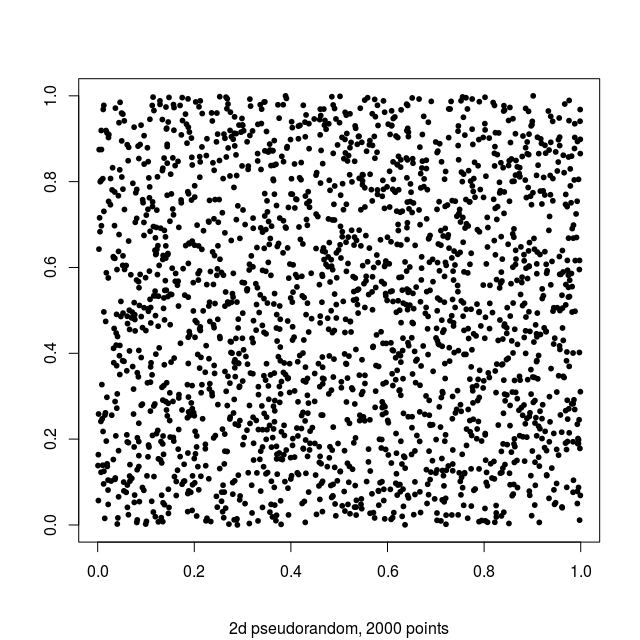
\includegraphics[width=0.5\linewidth]{figures/pseudo2d} 
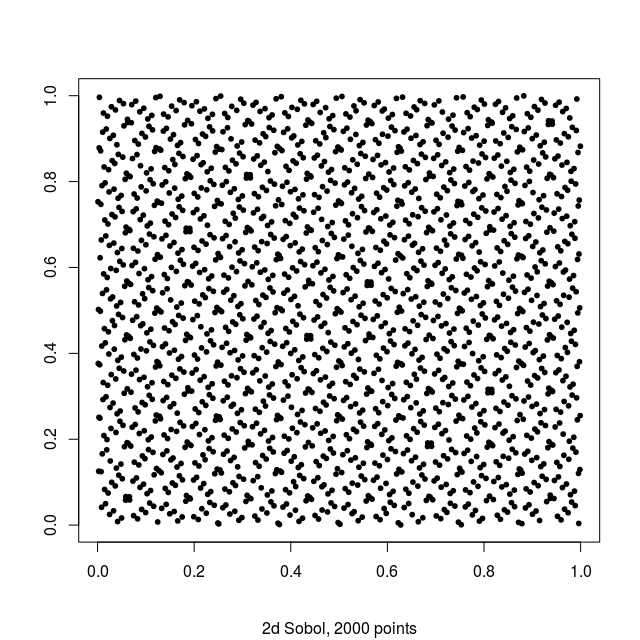
\includegraphics[width=0.5\linewidth]{figures/quasi2d} 
\caption{Bivariate uniform samples -  pseudorandom (left) and quasirandom (right).}
\label{fig:unnamed-chunk-1}
\end{figure}

Sobol sequences, as with other quasirandom sequences, have an inherent
dimensionality and a relatively short period - the sequence is exhausted
once every integer in the sample space has been sampled. Successive
samples evenly fill the sample space, and thus lack independence.
Conversely, a good pseudorandom generator has no discernible dependence
between variates often has a much longer period, allowing for very large
samples to be taken.

For applications such as numerical integration, Sobol sequences converge
at a rate of \(\approx1/N\) (actually \((ln N)^D/N\) (\cite{press_numerical_nodate})
compared to \(\approx1/\sqrt N\) for a pseudorandom generator, and thus
require far fewer samples to achieve the same level of accuracy. This makes quasirandom sampling particularly suitable for Monte-Carlo integration of high-dimensional functions: far fewer samples are required to obtain the same level of accuracy that would be achieved using pseudorandom sampling. 

Quasirandom sequences are not seeded like pseudorandom generators. To
avoid repetition, and for better degeneracy, it is recommended to
discard a number of variates on initialisation (\cite{joe_remark_2003}), and
on subsequent sampling continue the sequence from its previous position.

Consider the following simple example: we wish to calculate the expected value of the sum of 2 fair and independent dice, sampling 100 times. Using pseudorandom sampling, with a standard error proportional to the square root of the number of samples, we would expect to get an estimate of \(7 \pm 10\%\). However, using quasirandom sampling, since the standard error
\footnote{Strictly speaking, it is not mathematically valid to attribute a standard error value to results generated from a quasirandom sequence as there is no randomness. However the value is useful for qualitative comparison.} 
  is inversely proportional to the number of samples, the estimate will be \(7 \pm 1\%\). To achieve the same accuracy with peudorandom numbers would require 10000 samples.

When using quasirandom sequences it is extremely important to ensure that every sample is used. Discarding a subset of the samples will potentially destroy the statistical properties of the entire sequence. For this reason quasirandom sequences must not be combined with rejection sampling methods, which are often used to convert the 'raw' uniformly-distributed variates into e.g. normally-distributed ones.

%Think this example just adds confusion... For example, the \href{https://en.wikipedia.org/wiki/Ziggurat_algorithm}{Ziggurat algorithm} is a very efficient way of converting uniform variates to normally distributed ones, but it rejects a small proportion of the input 

\subsection{Sampling without Replacement}\label{sampling-without-replacement}

Given a discretely distributed population \(P\) of individuals which can be categorised into one of \(n\) states, each with integral frequencies
\(\{f_1,f_2,...f_n\}\), a random sample \(i \in \{1...n\}\) has
probability
\begin{equation}
p_i = \frac{f_i}{\sum\limits_{j=1}^{n}f_j}
\end{equation}
Once a sample \(i\) is taken the distribution is adjusted to
\(\{f_1,f_2,...f_i-1,...f_n\}\), with resultant impact on \(p\). Once
\(f_i\) has reached zero no further samples can take the value \(i\)
since \(p(i) = 0\).

Since \(f_i\) cannot be oversampled, this implies that all the other
states \(f_{j\neq{i}}\) cannot be undersampled. By extension, if all but
one states \(f_{i\neq{j}}\) cannot be oversampled, then \(f_j\) cannot
be undersampled. Thus each state can neither be under- nor oversampled:
the distribution must be matched exactly.

Extending this to two dimensions is straightforward: given marginal frequency vectors \(\mathbf{f}\) and \(\mathbf{g}\), each (for argument's sake) of length \(n\), and each summing to \(P\), take a random two dimensional sample \((i,j) \in \{1...n\}^2\) with probability
\begin{equation}
p_{i,j} = \frac{f_{i}g_{j}}{\sum\limits_{k=1}^{n}f_k\sum\limits_{k=1}^{n}g_k}
\end{equation}
and subseqently adjust values in each marginal vector
\begin{equation}
\begin{split}
f_i \leftarrow f_i-1 \\
g_j \leftarrow g_j-1 
\end{split}
\end{equation} 
This process can be repeated up to \(P\) times, when both marginal freqency vectors will be exhausted. The process 
extends easily to higher dimensions.

\subsection{Integerisation of Probabilities}\label{integerisation-of-probabilities}

Givena vector of discrete probabilities \(p_i\) for each state in a single category, and an overall population \(P\), the nearest integer frequencies \(f_i\) can be obtained using the following algorithm:
firstly obtain a lower bound for integer frequencies by computing
\begin{equation}
\begin{split}
f_i = \lfloor p_{i}P \rfloor \\
g_i = p_i P - f_i \\
X = P - \sum\limits_i{f_i}
\end{split}
\end{equation}
where \(g_i\) represents the difference between the unconstrained frequency and the integerised frequency and \(X\) is the shortfall in the integerised population. To remove the shortfall we simply increment the \(f_i\) corresponding to the largest \(X\) values of \(g_i\). This ensures that
\begin{equation}
\sum\limits_i{f_i} = P 
\end{equation}
matching the population, and that \(g_i\) is minimised. There may be multiple optimal solutions. 

\subsection{Problem Statement}\label{problem-statement}

Population synthesis (Orcutt 1957) refers to the (re)generation of
individual-level data from aggregate (marginal) data. For example, UK
census data provides aggregate data across numerous socio-economic
categories at various geographical resolutions - but it expressly does
not provide data at an individual-level, for privacy reasons among
others.

A mathematical statement of the problem is as
follows:\footnote{In the notation below, the index \(i\) is scalar and
  refers to a particular dimension. The index \(\mathbf{k}\) is a vector
  index \(\{k_1, k_2,...k_D\}\) of length \(D\), the dimensionality of
  the problem.}
we wish to generate a population \(P\) of individuals which can be characterised into \(D\) separate categories, 
each of which can occupy \(l\) discrete states. Each category is represented by a known frequency vector
\(\mathbf{m}_i\) of length \(l_i\) giving the marginal occurences of a state within a single category. 
Thus we have \(S\) possible overall states 
\begin{equation}
S=\prod\limits_{i=1}^{D}l_i
\end{equation}
and the aim is to populate a contingency table \(\mathbf T\) in \(D\) dimensions such that
\begin{equation}
\sum\limits_{\mathbf{k}, k_i fixed} \mathbf{T}_\mathbf{k} = \mathbf{m}_i
\label{eqn:margins}
\end{equation}
\begin{figure}[!t]
\centering
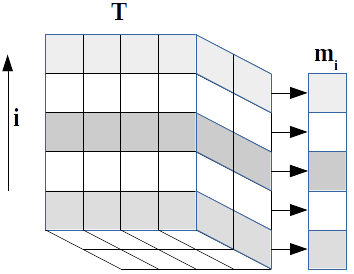
\includegraphics[width=0.35\linewidth]{figures/equation7} 
\caption{Illustration of the relationship between the contingency table \(\mathbf{T}\) and the marginal frequencies \(\mathbf{m}_i\), as expressed by equation \ref{eqn:margins}.}
\label{fig:eq7}
\end{figure} 
in other words each element of \(\mathbf{m}_i\) is the sum of all
elements in \(\mathbf{T}\) for a fixed value of \(k_i\). It is perhaps clearer to express this in visual form - see figure \ref{fig:eq7}. We define this as the \emph{marginal constraint}.

Each marginal sum and the sum of the elements of contingency table must
equal the population \(P\):
\begin{equation}
\sum\limits \mathbf{m}_{i} = \sum\limits_\mathbf{k} \mathbf{T} = P
\end{equation}
We define this as the \emph{population constraint}. 
Finally, the
\emph{integral constraint} restricts the elements to the natural
numbers:
\begin{equation}
{\mathbf{T} \in \mathbb{N}^S,\mathbf{m}_i} \in \mathbb{N}^{l_i}
\end{equation}

\begin{figure}[!t]
\centering
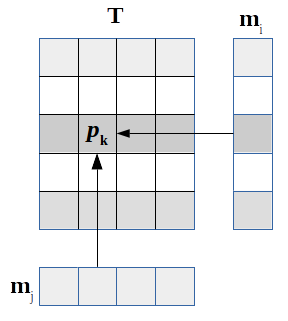
\includegraphics[width=0.35\linewidth]{figures/equation10} 
\caption{Illustration of the state probability defined in equation \ref{eqn:stateprob}.}
\label{fig:stateprob}
\end{figure}

The probability of a given state \(\mathbf{k}\) being occupied is thus
the product of the marginal probabilities:
\begin{equation}
p_{\mathbf{k}} = \prod\limits_{i=1}^{D}(\mathbf{m}_i)_\mathbf{k}/P
\label{eqn:stateprob}
\end{equation}
for which a two-dimensional example is illustrated for clarity in figure \ref{fig:stateprob}.
The degrees of freedom \(d\) of the system (required in order to
calculate the statistical significance of the population) is given by
\begin{equation}
d=\prod\limits_{i=1}^{D}(l_i-1)
\end{equation}
In the general case there are not enough constraints to determine a
unique solution. Hence there is a need to resort to iterative or
optimisation-type solutions, such as IPF, simulated annealing,
likelihood estimation, chi-squared fitting, or least-squares fitting.

\subsection{Degeneracy and Statistical
Likelihood}\label{degeneracy-and-statistical-likelihood}

In this work we interpret degeneracy as the number of possible different
ways a given overall population \(P\) can be sampled into a \(D\)-dimensional table
\(\mathbf{T}\) containing \(S\) possible states \(\mathbf{k}\), with
occupancy probability \(p_\mathbf{k}\), the system having \(d\) degrees
of freedom. Making the assumption that marginals are uncorrelated, then the
higher the degeneracy of the population, the more statistically likely
the population is.

We measure the degeneracy of populations using a \(\chi^2\) statistic:
\begin{equation}
\chi^2 = \sum\limits_{\mathbf{k}}\frac{(\mathbf{T}_\mathbf{k}-p_\mathbf{k}S)^2}{p_\mathbf{k}S}
\end{equation}
from which we can estimate a p-value, which represents the statistical
significance of the synthetic population.
\begin{equation}
\text{p-value}=1-F(d/2,\chi^2) 
\end{equation}
where \(F\) is the cumulative
\(\chi^2\) density function and \(d\) the degrees of freedom of the
system. The aim in this context is to generate populations with a high
p-value, i.e.~a low statistical significance and a high-degeneracy.

\section{The Algorithm}\label{the-algorithm}

This section describes the Quasirandom Integer Without-replacement Sampling (QIWS) algorithm. A commentary on the process by which we arrived at this algorithm follows in the Discussion.

\begin{enumerate*}
\item
  Create an \(D\)-dimensional discrete without-replacement distribution
  using the marginals \(\mathbf{m}_i\)
\item
  Sample \(P\) random variates from this distribution to create a
  population \(\mathbf{T}\). Specifically, we sample a value of
  \(\mathbf{k}\) and increment the value of \(\mathbf{T}_\mathbf{k}\),
  repeating until the distribution is fully depleted. Constructing the
  problem in this way automatically ensures that all constraints are
  automatically met, as explained in the previous section.
\item
  Compute occupation probabilities \(p_\mathbf{k}\) for each state
  \(\mathbf{k}\).
\item
  Compute a \(\chi^2\) statistic and a p-value, which represents the
  statistical significance of the synthetic population (in this case we
  prefer higher p-values, i.e.~statistically insignificant populations).
\end{enumerate*}

\subsection{The Implementation}\label{the-implementation}

The algorithm is implemented in an \texttt{R} package called
\texttt{humanleague}. A description of the technical implementation details can be found in the Appendix. The package is open source under a GPL licence and available at \url{https://github.com/CatchDat/humanleague}. It has been submitted for inclusion in the official CRAN repository of \texttt{R} packages.

In order to use this package, the input data requirements are a number of discrete integer marginal distributions, i.e. counts of population in each state of some category. If any marginal data is expressed as probabilities, a function is provided to convert these to integer frequencies.

\subsection{Usage Examples}\label{usage-examples}

\texttt{prob2IntFreq}: this function converts an array of discrete probabilities \(p_i\) into integral frequencies, given an overall population \(P\). It also returns the mean square error between the integer frequencies and their unconstrained values \(p_iP\).

\begin{Shaded}
\begin{verbatim}
> humanleague::prob2IntFreq(c(0.1, 0.2, 0.3, 0.4), 17)
$freq
[1] 2 3 5 7

$var
[1] 0.075
\end{verbatim}
\end{Shaded}

\texttt{synthPop}: This is function that performs the microsynthesis. The function supports dimensionalities up to 12, although this
limit is arbitrary and could be increased if necessary. Input is simply
a list of (between 2 and 12) integer vectors representing the marginals. Marginal vectors
must all sum to the population (to satisfy the population constraint) \(P\).
The output is broadly compatible with the established \texttt{mipfp}
(Barthelemy \& Suesse 2016) \texttt{R} package:
\begin{itemize*}
\item
  \(D\)-dimensional population table \(\mathbf{T_\mathbf{k}}\)
\item
  \(D\)-dimensional occupancy probability array
  \(\mathbf{p_\mathbf{k}}\)
\item
  boolean value indicating convergence
\item
  maximum value of each residual vector
\item
  \(\chi^2\) statistic
\item
  p-value
\end{itemize*} as can be seen by the example output below:
\begin{Shaded}
\begin{verbatim}
> x=c(10,10,10)
> p=humanleague::synthPop(list(x,x))
> p
$method
[1] "qiws"

$conv
[1] TRUE

$chiSq
[1] 1.2

$pValue
[1] 0.8780986

$error.margins
[1] 0 0

$p.hat
          [,1]      [,2]      [,3]
[1,] 0.1111111 0.1111111 0.1111111
[2,] 0.1111111 0.1111111 0.1111111
[3,] 0.1111111 0.1111111 0.1111111

$x.hat
     [,1] [,2] [,3]
[1,]    4    3    3
[2,]    4    3    3
[3,]    2    4    4
\end{verbatim}
\end{Shaded}

\texttt{sobolSequence}: this function simply produces a Sobol sequence of the requested dimension and length, optionally skipping part of the sequence. The example below produces the first ten values of the six-dimensional sequence, without skipping.
\begin{Shaded}
\begin{verbatim}
> humanleague::sobolSequence(6, 10)
        [,1]   [,2]   [,3]   [,4]   [,5]   [,6]
 [1,] 0.5000 0.5000 0.5000 0.5000 0.5000 0.5000
 [2,] 0.7500 0.2500 0.7500 0.2500 0.7500 0.2500
 [3,] 0.2500 0.7500 0.2500 0.7500 0.2500 0.7500
 [4,] 0.3750 0.3750 0.6250 0.1250 0.8750 0.8750
 [5,] 0.8750 0.8750 0.1250 0.6250 0.3750 0.3750
 [6,] 0.6250 0.1250 0.3750 0.3750 0.1250 0.6250
 [7,] 0.1250 0.6250 0.8750 0.8750 0.6250 0.1250
 [8,] 0.1875 0.3125 0.3125 0.6875 0.5625 0.1875
 [9,] 0.6875 0.8125 0.8125 0.1875 0.0625 0.6875
[10,] 0.9375 0.0625 0.5625 0.9375 0.3125 0.4375
\end{verbatim}
\end{Shaded}

\section{Comparison to Existing
Methods}\label{comparison-to-existing-methods}

\subsection{Statistical Properties}\label{statistical-properties}

For this we compared the QIWS algorithm to IPF using a number of
two-dimensional test cases. No integerisation was done to the IPF data (using e.g.~the \texttt{R}
package \texttt{rakeR}) due to that fact that integerisation can cause a
mismatch in one or more marginals.

IPF was initialised with a random seed array, each element uniformly
distributed in \([0,2)\), so that for the p-value tests the initial total population would be approximately equal to the final total.

The first three tests are made-up examples. The remainder are marginal
figures derived from 2011 UK census data at the MSOA level (mid-layer
super output area), with one dimension representing person status in
terms of age, sex, and economic activity, the other their workplace
location (MSOA).

\begin{table}[!t]
	\centering
	\begin{tabular}{c|c|c|c|c|c|c|c}
	\toprule
	Pop & States & N & QIWS \(\bar{c}\) & QIWS \(\bar{p}\) & IPF \(\bar{c}\) & IPF \(\bar{p}\)\tabularnewline
	\midrule
	20 & 4 & 1000 & 1 & 0.79 & 1 & 0.48\tabularnewline
	125 & 25 & 1000 & 1 & 0.91 & 1 & 0.06\tabularnewline
	935 & 49 & 1000 & 1 & 0.86 & 1 & 0.03\tabularnewline
	4958 & 16032 & 1000 & 1 & 0.81 & 1 & 1\tabularnewline
	4098 & 11760 & 1000 & 1 & 0.8 & 1 & 1\tabularnewline
	4029 & 11904 & 1000 & 1 & 0.8 & 1 & 1\tabularnewline
	4989 & 14640 & 1000 & 1 & 0.79 & 1 & 1\tabularnewline
	5219 & 15168 & 1000 & 1 & 0.79 & 1 & 1\tabularnewline
	\bottomrule
	\end{tabular}
	\caption{Convergence behaviour of population synthesis algorithms. \(N\)
	is the number of times the algorithm was run, \(\bar{c}\) refers to the
	convergence success rate, and \(\bar{p}\) refers to the mean p-value.}
	\label{tab1}	
\end{table}

A more detailed analysis was performed on two evenly distributed
marginal vectors of length 10 and a population \(P\) = 100 and number of
states \(S\) = 100, sampling 10000 populations.

For reference, the histogram of p-values using IPF (with random seed
values) yields the following rather unsurprising result\footnote{The IPF algorithm
 seeks to maximise entropy, resulting in a low \(\chi^2\) statistic (Lovelace et al. 2015).}:


\begin{figure}[!t]
\centering
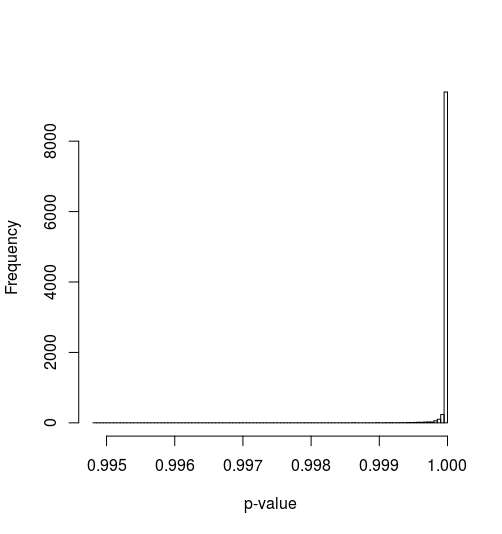
\includegraphics[width=0.5\linewidth]{figures/ipf_pvalue_dist}
\caption{Distribution of p-values of IPF.}
\label{fig2}
\end{figure}


We compared the statistical performance of our integer without-replacement sampling using a pseudorandom
generator and a quasirandom generator. The algorithm is guaranteed to
work in both cases so we looked at the distribution of p-values, which
can be seen in figure 3.

\begin{figure}[!t]
\centering
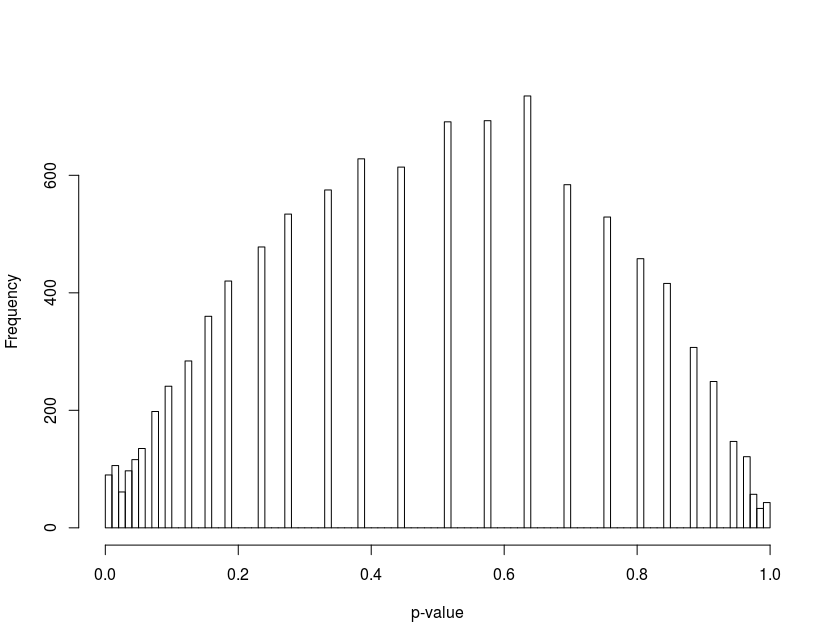
\includegraphics[width=0.498\linewidth]{figures/iqws_prng_pvalue_dist} 
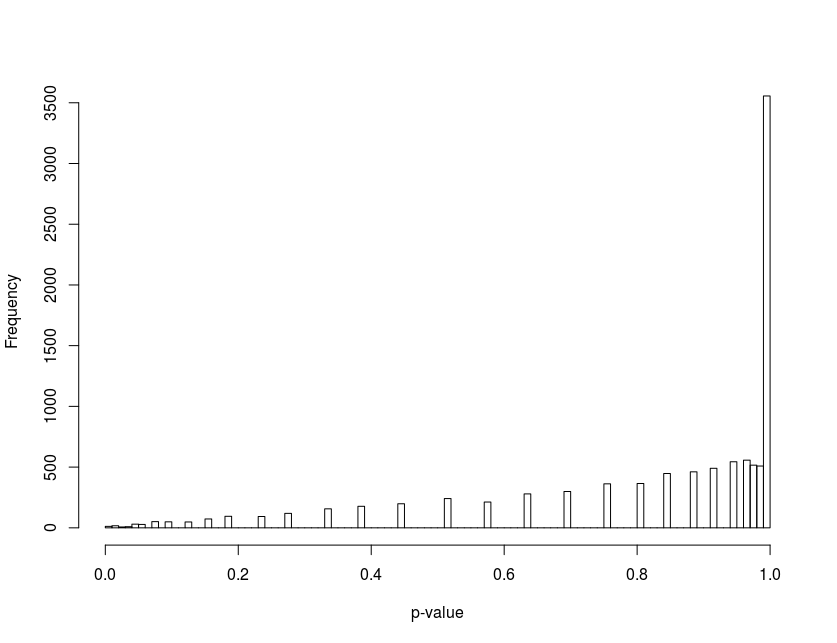
\includegraphics[width=0.498\linewidth]{figures/iqws_pvalue_dist} 
\caption{Distribution of p-values of QIWS using pseudorandom (left) and quasirandom (right) sampling.}
\label{fig:unnamed-chunk-4}
\end{figure}


\subsection{Performance}\label{performance}

Since computers vary widely in performance for many reasons, we present
normalised performance values.

\begin{table}[!t]
	\centering
	\begin{tabular}{c|c|c|c|c}
	\toprule
	Pop & States & N & QIWS & IPF\tabularnewline
	\midrule
	20 & 4 & 1000 & 1.0 & 66.3\tabularnewline
	125 & 25 & 1000 & 1.3 & 96.7\tabularnewline
	935 & 49 & 1000 & 2.3 & 68.3\tabularnewline
	4958 & 16032 & 1000 & 30.7 & 1559.3\tabularnewline
	4098 & 11760 & 1000 & 23.0 & 1069.0\tabularnewline
	4029 & 11904 & 1000 & 22.7 & 1027.3\tabularnewline
	4989 & 14640 & 1000 & 28.3 & 1457.0\tabularnewline
	5219 & 15168 & 1000 & 28.7 & 1557.7\tabularnewline
	\bottomrule			
	\end{tabular}
	\caption{Relative computation time of the algorithms for \(N\) runs, using the first case as a baseline.}
	\label{tab:}	
\end{table}

\section{Discussion}\label{discussion}

\subsection{Evolution of the
algorithm.}\label{evolution-of-the-algorithm.}

The motivation behind the development of this method came from the fact
that IPF, in general, does not generate integral populations in each
state. If the resulting population is used as a basis for Agent-Based
Modelling (ABM), then an integerisation process must be applied to the
synthesised population. Whilst this process preserves the overall
population, it may not exactly preserve all of the marginal
distributions. Although the integerisation process may not introduce significant errors, the
authors considered whether there was an alternative method of synthesis
that would directly result in an integral population that exactly
matched the marginal distributions.

We could not find any references in the literature on the use of
quasirandom sequences for the purpose of population synthesis, and so
decided to investigate the suitability of sampling algorithms using such
sequences.

Firstly, it was demonstrated that naive pseudorandom sampling could not
reliably generate populations matching the marginals. Since successive
samples are ostensibly independent, there is no mechanism to prevent
under- or oversampling of any particular state.

The initial algorithm simply sampled the marginal distributions (with
replacement), using quasirandom numbers, to build a population. For
``toy'' problems this method often worked, but for more complex problems
the algorithm often failed to exactly match all the marginals.

In general, the resulting population mismatched the marginals only
slightly. A correction algorithm was implemented which, applied at most
once for each dimension of the population, adjusted the states by the
error in the marginal for that dimension. This corrected the overall
population, and is reminiscent of an iteration in IPF.

It was also demonstrated that a correction step as described above could
not be applied to a pseudorandomly generated population because the
marginal errors were almost always too large to be able to apply a
correction: such corrections would typically result in a negative
population in one or more states.

Furthermore, it was shown that even using quasirandom sampling, it was
not always guaranteed that a population could be corrected using the
method described above without a negative population in one or more
states. The sparser (the ratio of the total population \(P\) to the
number of possible states \(S\)) the population, the more often this
would occur. Often the solution was simply to discard and resample the
population until an exact or correctable population was generated. This
raised a concern about the reliability (and efficiency) of the
algorithm, and in fact further testing did reveal cases where the
algorithm the number of resamples required was unacceptably large, even
exhausting the period of the generator.

This flaw drove the authors to come up with an alternative formulation
of the algorithm, and it transpired that without-replacement sampling
would guarantee that the population matched all marginals by design (as
explained in section 2.2), eliminating the need for the correction step
entirely. In fact, this method is guaranteed to work regardless of the
choice of underlying random number generation.

The next phase of the work was to analyse generated populations
statistically, focussing on the degeneracy of the resulting populations.
The results from this work, presented in the previous section, are
discussed below.

\subsection{Statistical Properties}\label{statistical-properties-1}

\subsubsection{General Remarks}\label{general-remarks}

Neither IPF nor QIWS failed to converge on any of the test cases in
Table 1.

One unexpected observation was that IPF performed least well on the
simple tests, generating the lowest mean p-values. Since these are
``toy'' examples we do not attribute any significance to this, putting
it down to our choice of random seed.

\subsubsection{Randomness in Context}\label{randomness-in-context}

To put pseudorandom versus quasirandom sampling into context, consider a
``random'' number generator that simply always returns zero. If we used
this as the basis for without-replacement sampling of a marginal
distribution \(\lbrace10,10,10\rbrace\), we would get a sequence
consisting of ten ones, ten twos and ten threes as the samples exhausted
each bin and moved to the next. In two dimensions, this would result in
a population matrix
\[\left( \begin{array}{ccc}
10 & 0 & 0 \\
0 & 10 & 0 \\
0 & 0 & 10 \end{array} \right)\]
suggesting that the marginals are strongly correlated. This particular
result has a low degeneracy - there are relatively few different ways at
arriving at this result - and a p-value of effectively zero implying
that it is vanishingly unlikely that this population resulted by chance.

\subsubsection{Degeneracy}\label{degeneracy}

The \(\chi^2\) value resulting from IPF is likely to be slightly lower
than QIWS due to the fact the former numbers are not generally integral.
Figure 2 demonstrates that IPF almost always results in a p-value of 1.
This is entirely expected due to the fact that the IPF algorithm seeks a 
maximum-entropy solution.

QIWS does not achieve such high p-values in general, as seen in figure
3, and there is a marked difference in the distribution of p-values
depending on the type of underlying random generator used. It can be
seen clearly that quasirandom sampling generally yields more degenerate
populations, and is much closer to IPF in this respect.

It should be borne in mind that one of the reasons that QIWS cannot
achieve the high p-value levels as consistently as IPF is due to the
simple fact that the population is integral, and this will generally
result in a higher \(\chi^2\) statistic. We would caution users,
however, to check the resulting p-value against some suitable threshold
and resample if necessary.

\subsection{Performance}\label{performance-1}

QIWS performance is far superior to IPF. One reason for this is that
QIWS is not iterative, but the following points should be noted:

\begin{itemize*}
\item
  the comparison is somewhat unfair since our implementation is compiled
  \texttt{C} and \texttt{C++} code and Ipfp's implementation is
  interpreted \texttt{R} code.
\item
  performance of population synthesis may not be a significant factor in
  most workflows, and thus speed may be of marginal advantage. However
  in large-scale ensemble simulation applications, the performance of
  QIWS may be an advantage.
\end{itemize*}

\subsection{Application / Range of Use}\label{application-range-of-use}

IPF can be used for microsimulation in cases where some marginal data is
not fully specified. For example, some categorical constraint data may
only be available for a subset of the whole population. By using this
data in the initial guess for the iteration, rather than as a marginal
constraint, the incomplete data is scaled to, and smoothed over, the
overall population. An example of this type of microsimulation
``CakeMap'' is given in Lovelace and Dumont (2016).

QIWS requires that all marginals are fully-specified. It needs this data
to construct a multivariate discrete distribution to sample from. It is
thus not applicable to problems such as ``CakeMap''.

For agent-based modelling (ABM) applications, QIWS has the advantage
that it always generates integer populations. Thus integerisation, which
may alter the population in such a way that the marginals are no longer
met, is not required.

QIWS may potentially be of use in the process of anonymising
populations. It is outside the scope of this work, but since full
marginal data will likely be available, its use in this context may be
worth investigating.

\section{Conclusion}\label{conclusion}

This work forms part of a larger project in which a city-scale
population microsynthesis is used as the basis for an Agent-Based Model
of commute patterns, using census data combined with a crowdsourced
dataset. The QIWS algorithm and the software implementation in an
\texttt{R} package was developed for this purpose, eliminating the need
for integerising the synthesised population. This microsimulation
involved categorical variables (i.e.~marginals) representing home and
work locations (at MSOA resolution), mode of transport, gender, age
group, and economic activity type, with the crowdsourced data overlaid
on the larger census population.

The QIWS algorithm was thus designed with this type of synthesis in
mind, where all marginal data is fully specified, and in this context it
fulfils the requirements.

If there are specific requirements for a degenerate population,
statistical data is provided about the generated population that will
guide the user in determining the suitability of the generated
population.

In situations where integral populations are desirable QIWS presents an
advantage over established techniques by eliminating the need for
postprocessing the population - for instance by integerisation.

In applications where performance is a key factor, we have shown that
our implementation of QIWS comfortably outperforms a popular \texttt{R}
implementation of IPF (Barthelemy and Suesse 2016). For large-scale
ensemble modelling, this could be advantageous.

We have established that QIWS can be used for microsynthesis given
aggregate data. Although outside the scope of this work, we believe that
the algorithm could equally be applied to an anonymisation process
whereby individual-level data is first aggregated and then synthesised,
for example (Nowok, Raab, and Dibben 2016).

We are aware that QIWS is more limited in scope than IPF in that it is
unable to deal with cases where some marginal data is not explicitly
specified, instead being expressed in the seed population used to
initialise the IPF iteration. It may be that with further development of
the algorithm some of these limitations could be overcome.

As such we envisage QIWS as a technique that complements rather than
supplants established methods, and publicise the technique as such.

\section{Acknowledgements}\label{acknowledgements}

The authors acknowledge Innovate UK's Catch! project for providing the
funding for this work.

%%%%%%%%%%%%%%%%%%%%%%%%%%%%%%%%%%%%%%%%%%%%%%

% FIGURES AND TABLES

% Figures should be placed in the desired position within the text. Please follow the template below.
% Figure widths can be set using absolute dimensions (e.g., [width = 12cm]) or relative ones (e.g., [width = 0.8/textwidth]). We strongly suggest to use the latter option, as this allows automatic adaptation to different paper widths

%\begin{figure}[!t]
%\centering
%\includegraphics[width=????\textwidth]{????}
%\caption{}
%\label{fig:????}
%\end{figure}

% Tables should be placed in the desired position within the text. Please follow the template below

%\begin{table}[!t]
%	\centering
%	\begin{tabular}{????}
%	\toprule
% 	% first line
%	\midrule
%	% tale body	
%	\bottomrule			
%	\end{tabular}
%	\caption{}
%	\label{tab:????}	
%\end{table}

%%%%%%%%%%%%%%%%%%%%%%%%%%%%%%%%%%%%%%%%%%%%%%
% End of  paragraph numbering. Please leave this untouched
\endparano

%%%%%%%%%%%%%%%%%%%%%%%%%%%%%%%%%%%%%%%%%%%%%%

%%%%%%%%%%%%%%%%%%%%%%%%%%%%%%%%%%%%%%%%%%%%%%

% APPENDICES
% Put your appendices here. Please use the normal sectioning command, e.g.,
% \section{Appendix A: <title of the appendix>}
% \section{Appendix B: <title of the appendix>}
% ...

\section{Appendix: Implementation - Technical Detail} 
The algorithm is implemented in an \texttt{R} package called
\texttt{humanleague}, written in \texttt{C++11} and \texttt{C} and
exposed to \texttt{R} via \texttt{Rcpp}. We used open source
implementations of the Sobol sequence generator (\cite{johnson_stevengj/nlopt:_nodate}) and, in order to 
compute the p-value, the
incomplete gamma function (\cite{burkardt_asa032_2008})

One of the many useful features introduced in \texttt{C++11} was a
standard random number framework, which splits underlying (uniform) generators
and the distributions, and defines APIs that these classes should
implement \href{http://en.cppreference.com/w/cpp/numeric/random}{(see
e.g. http://en.cppreference.com/w/cpp/numeric/random)}. There is no
native support for quasirandom generators nor for without-replacement
distributions, but by conforming to the APIs they can be implemented to
interoperate with the native generator and distribution implementations.

It should be noted that there are two instances where the new types
extend the standard interfaces (see class definitions below):

\begin{itemize*}
\item
  a quasirandom generator has inherent dimensionality, and thus should
  return that number of variates per sample. In our implementation we
  provided both the standard single-valued \texttt{operator()} and the
  extended vector \texttt{buf()} accessor functions.
\item
  without-replacement sampling will eventually become exhausted, as a
  result we provided a boolean \texttt{empty()} function to check if the
  distribution is exhausted. If exhausted, the accessor functions will
  throw an exception.
\end{itemize*}

The Sobol sequence generator is implemented in such a way that it is not reset
each time a population is requested, allowing different populations to
be generated each time, up to the limit of the sequence being exhausted.
Our implementation uses 32-bit unsigned integers, thus allowing for
\(\approx4\times10^9\) samples (in each dimension).

\begin{Shaded}
\begin{Highlighting}[]
  \KeywordTok{class} \NormalTok{Sobol}
  \NormalTok{\{}
  \KeywordTok{public}\NormalTok{:}
    \KeywordTok{typedef} \DataTypeTok{uint32_t} \NormalTok{result_type;}
    \KeywordTok{explicit} \NormalTok{Sobol(}\DataTypeTok{uint32_t} \NormalTok{dim, result_type nSkip = }\DecValTok{0u}\NormalTok{);}
    \NormalTok{~Sobol();}
    \DataTypeTok{const} \NormalTok{std::vector<result_type>& buf();}
    \NormalTok{result_type }\KeywordTok{operator}\NormalTok{()();}
    \DataTypeTok{void} \NormalTok{skip(result_type n);}
    \NormalTok{result_type min() }\DataTypeTok{const}\NormalTok{;}
    \NormalTok{result_type max() }\DataTypeTok{const}\NormalTok{;}
  \KeywordTok{private}\NormalTok{:}
    \NormalTok{SobolData* m_s;}
    \DataTypeTok{uint32_t} \NormalTok{m_dim;}
    \NormalTok{std::vector<result_type> m_buf;}
    \DataTypeTok{uint32_t} \NormalTok{m_pos;}
  \NormalTok{\};}

  \KeywordTok{template}\NormalTok{<}\KeywordTok{typename} \NormalTok{I> }\CommentTok{// I must be an integral type}
  \KeywordTok{class} \NormalTok{discrete_distribution_without_replacement}
  \NormalTok{\{}
  \KeywordTok{public}\NormalTok{:}
    \KeywordTok{typedef} \NormalTok{I result_type;}
    \CommentTok{// enforce integral types only}
    \KeywordTok{static_assert}\NormalTok{(std::is_integral<I>::value, }
      \StringTok{"discrete_distribution_without_replacement: only integral types supported"}\NormalTok{);}
    \NormalTok{discrete_distribution_without_replacement(}\KeywordTok{typename} \NormalTok{std::vector<I>::const_iterator b, }
                                              \KeywordTok{typename} \NormalTok{std::vector<I>::const_iterator e);}
    \CommentTok{// std::distribution compatibility}
    \KeywordTok{template}\NormalTok{<}\KeywordTok{typename} \NormalTok{R>}
    \NormalTok{result_type }\KeywordTok{operator}\NormalTok{()(R& rng);}
    \NormalTok{result_type }\KeywordTok{operator}\NormalTok{()(result_type r);}
    \DataTypeTok{bool} \NormalTok{empty() }\DataTypeTok{const}\NormalTok{;}
  \KeywordTok{private}\NormalTok{:}
    \NormalTok{std::vector<I> m_freq;}
    \NormalTok{I m_sum;}
  \NormalTok{\};}
\end{Highlighting}
\end{Shaded}


%%%%%%%%%%%%%%%%%%%%%%%%%%%%%%%%%%%%%%%%%%%%%%

% ENDNOTES. Please uncomment the line below in case of notes.
% \theendnotes

%%%%%%%%%%%%%%%%%%%%%%%%%%%%%%%%%%%%%%%%%%%%%%

% REFERENCES.
% The JASSS bibliographic style file (jasss.bst) is included in the bundle. Please use BibTeX, not BibLaTeX.
% Use natbib commands for references (\citep{}, \citet{}, etc.), not standard LaTeX ones (\cite{}).
% Remember to include the doi and url fields in your bib database. The address field should be included for books.
% Please upload the bib file (not just the bbl one) when submitting.
 
\bibliographystyle{jasss}
\bibliography{./ref.bib} % Please set the right name for your bib file

%%%%%%%%%%%%%%%%%%%%%%%%%%%%%%%%%%%%%%%%%%%%%%

\end{document}